\documentclass{exam}
\usepackage[utf8]{inputenc}
\usepackage{lmodern}
\usepackage{microtype}

% \usepackage[parfill]{parskip}
\usepackage[dvipsnames]{xcolor}
\usepackage{amsmath}
\usepackage{amsfonts}
\usepackage{amsthm}
\usepackage{siunitx}
\DeclareSIUnit\year{yr}
\DeclareSIUnit\foot{ft}
\DeclareSIUnit\litre{\liter}

\usepackage{skull}

\usepackage{pgfplots}
\usepgfplotslibrary{polar}
\pgfplotsset{compat=1.11}
\usepgfplotslibrary{statistics}
\usepackage{graphicx}
\usepackage{sidecap}
\sidecaptionvpos{figure}{c}
\usepackage{float}
\usepackage{gensymb}
\usepackage{tkz-euclide}
\usetkzobj{all}
\usepackage{commath}
\usepackage{hyperref}
\usepackage{enumitem}
\usepackage{wasysym}
\usepackage{multicol}
\usepackage{mathtools}
\usepackage{tcolorbox}
\usepackage{tabularx}
\usepackage[version=4]{mhchem}
\usepackage{changepage}
\usepackage{listings}
\lstset{basicstyle=\ttfamily\linespread{0.8}\small}

\renewcommand*{\thefootnote}{\fnsymbol{footnote}}

\newtheorem*{thm}{Theorem}
\newtheorem*{iden}{Identity}
\newtheorem*{lemma}{Lemma}
\newtheorem{obs}{Observation}
\theoremstyle{definition}
\newtheorem*{defn}{Definition}
\newtheorem*{ex}{Example}
\newtheorem{con}{Construction}
\newtheorem*{alg}{Algorithm}

\newtheoremstyle{break}
  {\topsep}{\topsep}%
  {\itshape}{}%
  {\bfseries}{}%
  {\newline}{}%
\theoremstyle{break}
\newtheorem*{bthm}{Theorem}

% russian integral
\usepackage{scalerel}
\DeclareMathOperator*{\rint}{\scalerel*{\rotatebox{17}{$\!\int\!$}}{\int}}

% \DeclareMathOperator*{\rint}{\int}

\pgfplotsset{vasymptote/.style={
    before end axis/.append code={
        \draw[densely dashed] ({rel axis cs:0,0} -| {axis cs:#1,0})
        -- ({rel axis cs:0,1} -| {axis cs:#1,0});
    }
}}

% \pointsinrightmargin
\boxedpoints
\pointname{}

\newcommand{\questioA}{\question[\texttt{\textbf{\color{Cerulean} A}}]}
\newcommand{\questioM}{\question[\texttt{\textbf{\color{PineGreen} M}}]}
\newcommand{\questioE}{\question[\texttt{\textbf{\color{WildStrawberry} E}}]}
\newcommand{\questioS}{\question[\texttt{\textbf{\color{Goldenrod} S}}]}
\newcommand{\questioO}{\question[\texttt{\textbf{\color{BurntOrange} O}}]}

\newcommand{\parA}{\part[\texttt{\textbf{\color{Cerulean} A}}]}
\newcommand{\parM}{\part[\texttt{\textbf{\color{PineGreen} M}}]}
\newcommand{\parE}{\part[\texttt{\textbf{\color{WildStrawberry} E}}]}
\newcommand{\parS}{\part[\texttt{\textbf{\color{Goldenrod} S}}]}
\newcommand{\parO}{\part[\texttt{\textbf{\color{BurntOrange} O}}]}

\newcommand{\subparA}{\subpart[\texttt{\textbf{\color{Cerulean} A}}]}
\newcommand{\subparM}{\subpart[\texttt{\textbf{\color{PineGreen} M}}]}
\newcommand{\subparE}{\subpart[\texttt{\textbf{\color{WildStrawberry} E}}]}
\newcommand{\subparS}{\subpart[\texttt{\textbf{\color{Goldenrod} S}}]}
\newcommand{\subparO}{\subpart[\texttt{\textbf{\color{BurntOrange} O}}]}

\newcommand{\mainHeader}[2]{\section*{NCEA Level 2 Mathematics\\#1. #2}}
\newcommand{\mainHeaderHw}[2]{\section*{NCEA Level 2 Mathematics (Homework)\\#1. #2}}
\newcommand{\seealso}[1]{\begin{center}\emph{See also #1.}\end{center}}
\newcommand{\drills}[1]{\begin{center}\emph{Drill problems: #1.}\end{center}}
\newcommand{\basedon}[1]{\begin{center}\emph{Notes largely based on #1.}\end{center}}

\begin{document}

\section*{NCEA Level 3 Calculus\\Introduction to the Notes}

\begin{center}
  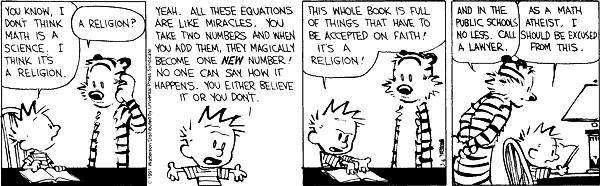
\includegraphics[width=0.8\textwidth]{hobbes}
\end{center}

\subsection* {What is Calculus?}
I will refrain from trying to advertise the subject to you, and will simply try to explain what calculus is and what kind of
person uses it. Calculus is the broad study of:
\begin{itemize}
  \item Continuous change;
  \item Slope, area, and volume; and
  \item Functions and relationships.
\end{itemize}

It has applications in physics, where calculus is the most natural language for Newtonian mechanics and classical electromagnetism; in chemistry
and biology, where calculus can be used to model anything which changes over time (like rates of reaction, concentrations, and populations); in
statistics (the study of probability distributions is just calculus); and in economics (I am assured). My own view, which I try to sprinkle throughout
these notes, is mainly a mixture of geometric applications and physical intuition.

Within mathematics itself, calculus is the computational side of \textbf{real analysis}, the study of the properties of the real number system.

\subsection*{Mathematical Prerequisites}
There are a number of things from Level 2 Mathematics that students should be
comfortable with; generally, I assume in these notes a vague merit-level understanding
of the core level 2 standards (by which I mean, the reader should be comfortable solving
achieved level problems without guidance and have some idea how to approach more difficult
problems):
\begin{itemize}
  \item Level 2 Algebra: All material on quadratics (factorising, solving, discriminants), logs and exponents.
  \item Level 2 Calculus: Basic differentiation, geometric meaning of derivative (in particular, integration is \textit{not} assumed)
  \item Level 2 Graphing: Recognising $ x-$/$ y-$shift of general functions, slope-intercept and point-slope form of linear equations,
                          recognising period/frequency/amplitude/$ x-$/$ y-$shift from a trig function.
  \item Level 2 Trigonometry: Trig ratios, the Pythagorean theorem.
  \item Level 2 Simultaneous Equations: Solving linear and quadratic simultaneous equations.
  \item Level 2 Co-ordinate Geometry: Distances and linear equations.
\end{itemize}

Further into the notes, I also touch a bit on concepts covered in some of the other Level 3 standards,
but not in so much detail that they need to be covered first:
\begin{itemize}
  \item Level 3 Conics: Recognising forms from equations.
  \item Level 3 Algebra: Surds.
  \item Level 3 Trigonometry: Solving trig equations (including general solutions), reciprocal trig functions, use
                              of trig identities (this latter mainly for E/S/OS-style integration problems).
\end{itemize}
In particular, no knowledge of complex algebra is assumed (or used) anywhere in the notes, and no knowledge from any L2 or L3 statistics standards is assumed.

I also do expect the reader to be able to draw graphs various simple functions (e.g. parabolae, the three basic trig functions, logs and
exponents, and so forth) `by eye' --- I realise that this is a little unrealistic, but at some point one must learn to become comfortable
with the shapes and sizes of the objects we study. In order to help build this intuition, it is (very highly) recommended that the reader
works through every example in detail, drawing pictures and so forth.

\subsection*{A Note on Problem Difficulty}
One of the main goals for these notes is that they should be useful for students at all levels, from A to OS. Accordingly, the
problems each week range from simple (most students should be able to just write down an answer without thinking too hard) to
extremely non-trivial (it took \textbf{me} a while to work the problem, and I know this material quite well). If you can't do
a problem, the best thing to do is to move on and come back to it --- the problems don't always increase in difficulty. Of course,
it is important to do a good number of problems \textbf{including some difficult ones}; you're not under exam conditions here
and you're going to get an awful lot more out of a hard problem than an easy one!

I have marked the problems in the weekly worksheets (\textbf{not} the homework) with symbols relating vaguely to difficulty:

\begin{center}
\texttt{\textbf{\color{Cerulean} A}}
\texttt{\textbf{\color{PineGreen} M}}
\texttt{\textbf{\color{WildStrawberry} E}}
\texttt{\textbf{\color{Goldenrod} S}}
\texttt{\textbf{\color{BurntOrange} O}}
\end{center}

However, these are for my own reference and should not be taken to be accurate with respect to actual examinations.

\subsection*{Required content for Level 3}
Some of the material goes beyond that required for NCEA Level 3; the following list gives some idea of the level of each sheet.

\subsubsection*{Differentiation}
\begin{enumerate}
  \item[01.] The Derivative
  \item[02.] Limits
  \item[03.] Derivatives of Common Functions
  \item[04.] The Chain Rule
  \item[05.] The Product and Quotient Rules
  \item[06.] Tangent and Normal Lines
  \item[07.] The Geometry of Functions
  \item[08.] Optimisation
  \item[09.] Implicit Differentiation
  \item[10.] $^*$Inverse Functions
  \item[11.] Related Rates of Change
  \item[12.] Parametric Functions
  \item[13.] $^{*\perp}$Sequences and Series
  \item[14.] $^\dagger$Differentiation Revision
\end{enumerate}

\subsubsection*{Integration}
\begin{enumerate}
  \item[15.] Approximating Areas
  \item[16.] Anti-differentiation
  \item[17.] The Fundamental Theorem of Calculus
  \item[18.] Substitution
  \item[19.] Differential Equations
  \item[20.] $^*$Partial Fractions
  \item[21.] $^*$Integration by Parts
  \item[22.] $^{*\perp}$Lengths, Volumes, and Areas
  \item[23.] $^*$Trigonometric Substitution
  \item[24.] $^\perp$Kinematics
  \item[25.] $^\dagger$Integration Revision
  \item[26.] $^{*\perp\dagger\skull}$More Interesting Problems
\end{enumerate}

($^*$scholarship topic, $^\perp$interest topic, $^\dagger$revision, $^\skull$reader discretion advised)

\subsection*{A Note on the Textbook}
Many problems are taken from a couple of places:
\begin{itemize}
  \item Stewart's Calculus (the current trendy textbook)
  \item Anton's Calculus (the old trendy textbook)
  \item Spivak's Calculus (the textbook you should use)
  \item University of Canterbury MATH199 lecture notes and problem sets
  \item Old NCEA/Scholarship exams
\end{itemize}
Most textbooks cover all the relevant material in the first few chapters (the first five or so in Stewart).

\subsection*{Homework}
Every week has an associated homework sheet with a page of reading (five minutes or so) and a few questions (generally all
pretty straightforward, but there is often a challenge question on there to keep you occupied).

I cannot emphasise enough how important it is to \textbf{do the homework}.

\subsection*{How to Read Mathematics}
\begin{center}
  \textit{So we shall now explain how to read the book. The right way is to put it on your desk in the day, below your pillow at night, devoting yourself to the reading, and solving the exercises till you know it by heart. Unfortunately, I suspect the reader is looking for advice on how not to read, i.e. what to skip, and even better, how to read only some isolated highlights.}\\ - Saharon Shelah, `Classification Theory and the Number of Non-Isomorphic Models'
\end{center}

A major part of Level 3 Mathematics is preparation for university-level study in pure mathematics or the hard or soft sciences. As such, this
year we begin to expose you to some `real mathematics' --- not just the watered-down calculation and computation you've been doing since intermediate,
but a real journey of discovery through one of humanity's great fields of human experience. I guarantee that at primary school you enjoyed
this kind of mathematics --- for example, consider the non-obvious fact that $ 3 \times 5 = 5 \times 3 $. Next year you will learn that there are
some objects which do not have this property (commutativity).

There are a lot of definitions and theorems, but they allow us to capture our intuition of mathematical objects, and their behaviour in a more
precise (and more correct) sense. It is important to read slowly and understand the statements as you go, as every piece strengthens the whole.
I do not tend to repeat myself, so often you will find statements from earlier used later without comment.

I have also included proofs of a few of the theorems that we use, but rigorous proofs of many seemingly obvious ideas (like the fact that every function
reaches a minimum and a maximum value on any closed interval) require some subtle properties of the real numbers and so it is more important to gain a
geometric and intuitive feeling for many of the results rather than worrying too much.

\textbf{Recommended reading for the interested}: Paul Lockhart's `A Mathematician's Lament'.

\end{document}
